\documentclass{beamer} 
\usepackage{multicol}
\usepackage{url}

\title{(Non) Comprehensive Guide to C/C++ Source Code Quality} 
\author{Sergey Kishchenko} 
\date{March 25th, 2011} 
\usetheme{CambridgeUS}
\usecolortheme{seagull}
\institute{Quickoffice}
\begin{document}

\frame{\titlepage}
\begin{frame} 
\frametitle{Product quality and source code Quality}
\begin{multicols}{2}
\center{Source code}

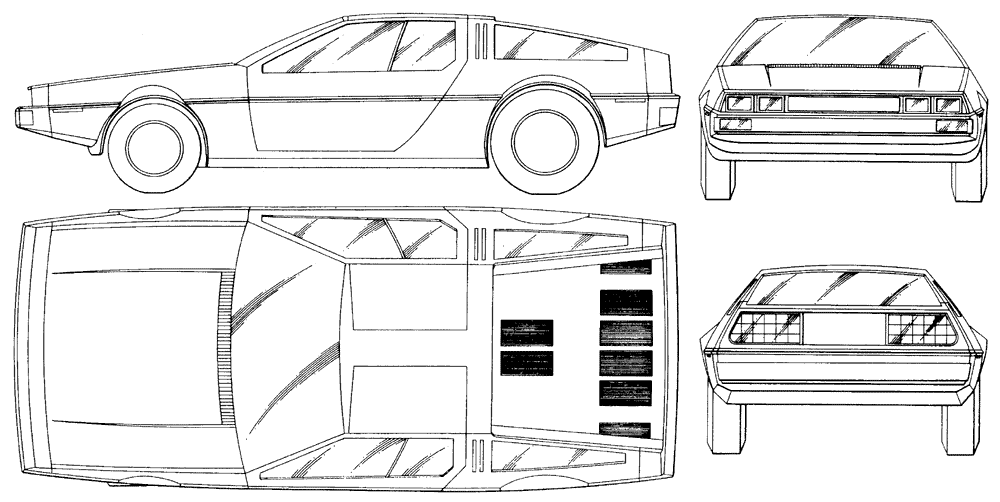
\includegraphics[width=0.4\textwidth]{img/delorean-blueprint}
\columnbreak
\center{Product}

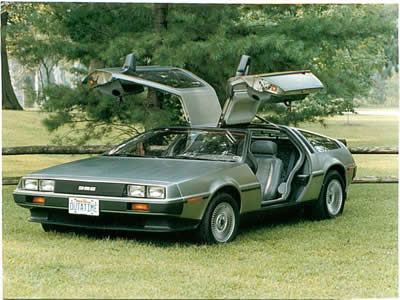
\includegraphics[width=0.4\textwidth]{img/delorean}
\end{multicols}
\begin{center}
\textbf{You can't make a good quality product with bad quality blueprint!}
\end{center}
\end{frame} 

\begin{frame}
\frametitle{Software product quality}
\begin{itemize}
\item Conformance to the specification
\item Completeness
\item Product documentation
\item \textbf{Source code quality}
\end{itemize}
\end{frame}

\begin{frame}
\frametitle{Source code quality}
\begin{itemize}
\item Correctness(no "bugs"!)
\item Maintainability
\item Readability
\item Portability
\item Low complexity
\item High code reuse
\item Efficiency
\end{itemize}
\end{frame}

\begin{frame}
\frametitle{Measuring source code quality}
\begin{itemize}
\item Bugs per line of code
\item Number of lines of code
\item Conformance to the code styling guide
\item Amount of platform-dependent code
\item Code coverage
\item Comment density
\item Program execution time, program size
\end{itemize}
\begin{center}
\textbf{There is no "silver bullet" source code quality metric :(}

\textbf{You should choose some of the points above and produce your own integral metric.}
\end{center}
\end{frame}

\begin{frame}
\begin{block}{\begin{center}\Large\textbf{How to measure and improve source code quality}\end{center}}
\begin{center}
\textbf{Part 1. Tools}
\end{center}
\end{block}
\end{frame}

\begin{frame}
\frametitle{CPD(Copy/Paste detection)}
\begin{center}
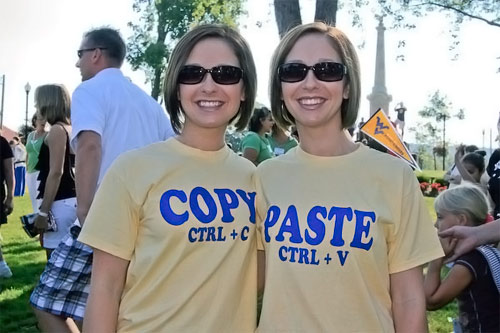
\includegraphics[width=0.4\textwidth]{img/copy-paste}
\end{center}
Improves readability, maintainability, increases code reuse, reduces resources usage. You can download it at \url{http://pmd.sourceforge.net/cpd.html}
\begin{exampleblock}{How to use}
java net.sourceforge.pmd.cpd.CPD --minimum-tokens 100 --files /path/to/cpp/source --language cpp
\end{exampleblock}
\end{frame}

\begin{frame}
\frametitle{gcc -Wall -ansi -pedantic}
I'm serious, it is one of the best tool you can get. Do not underestimate it.
\begin{exampleblock}{How to use}
gcc -Wall -ansi -pedantic -c /path/to/source/file.cpp
\end{exampleblock}
\end{frame}

\begin{frame}
\begin{block}{\begin{center}\Large\textbf{How to measure and improve source code quality}\end{center}}
\begin{center}
\textbf{Part 2. General ideas}
\end{center}
\end{block}
\end{frame}

\begin{frame}
\frametitle{Code review}
Improves correctness, readability, maintainability
\begin{exampleblock}{How to use}
\end{exampleblock}
\end{frame}



\end{document}
